\documentclass[10pt,a4paper,openany,twoside, prof]{book}

\usepackage{layout_cours}

\begin{document}

\chapnumber{14} % numéro du chapitre
\titre{Probabilités} % titre du chapitre
\classe{Seconde} % classe
\entetegal
% 
% \paragraph*{Objectif du chapitre :}
% \begin{itemize}
% \item  Connaître et utiliser le vocabulaire univers, expérience aléatoire, événement, éventualité et issues.
% \item  Comprendre et interpréter un événement contraire, une intersection ou réunion d'événements.
% \item  Reconnaître et utiliser une situation d'équiprobabilité.
% \item  Calculer des probabilités à l'aide d'une distribution de fréquences, d'un arbre des possibles ou d'un tableau.
% \end{itemize}

\section{Vocabulaire des événements} 

\begin{defi}{Issue, univers}{}
   Chaque résultat possible d'une expérience aléatoire est appelé \textbf{issue} ou \textbf{éventualité}. C'est une description mathématique des possibilités.

   L'ensemble formé par les issues est appelé \textbf{univers}, il est très souvent noté $\Omega$.
\end{defi}

\begin{ex}{}{}
   \begin{itemize}
      \item  Lancer d'une pièce de monnaie : $\Omega =\{$~pile~;~face~$\}$,
      \item  lancer un dé à six faces : $\Omega =\{~1~;~2~;~3~;~4~;~5~;~6~\}$.
   \end{itemize}
\end{ex}

\begin{defi}{}{}
   \begin{itemize}
      \item  Un \textbf{événement} de l'expérience aléatoire est une partie quelconque de l'univers.
      \item  Un événement ne comprenant qu'une seule issue est un \textbf{événement élémentaire}.
   \end{itemize}
\end{defi}

\begin{ex}{Evénement}{}
   \begin{itemize}
      \item  $A$ : \og obtenir un $5$ \fg{} est un événement élémentaire correspondant à $A=\{~5~\}$,
      \item  $B$ : \og obtenir un numéro pair \fg{} est un événement correspondant à $B=\{~2~;~4~;~6~\}$.
   \end{itemize}
\end{ex}

\begin{defi}{Evénement élémentaire, événement certain}{}
   \begin{itemize}
      \item  L'événement qui ne contient aucune issue est l'\textbf{événement impossible}, noté $\varnothing$,
      \item  l'événement composé de toutes les issues est appelé \textbf{événement certain}.
   \end{itemize}
\end{defi}

\begin{ex}{}{}
   \begin{itemize}
      \item  Tirage des six numéros gagnants du loto : \og obtenir la combinaison $3-25-38-59-67-91$ \fg{} est un événement impossible (les numéros vont de $1$ à $49$),
      \item  Lancer d'un dé à six faces : \og obtenir un nombre positif \fg{} est un événement certain.
   \end{itemize}
\end{ex}

\begin{defi}{Evénement contraire}{}
   Pour tout événement $A$ il existe un événement noté $\overline{A}$ et appelé \textbf{événement contraire} (ou complémentaire) de $A$, qui est composé des éléments de $\Omega$ qui ne sont pas dans A.
\end{defi}

\begin{ex}{}{}
   \begin{itemize}
      \item  Lancer d'une pièce de monnaie : si $A=\{\text{~pile~}\}$ alors son événement contraire est $\overline{A}=\{\text{~face~}\}$,
      \item  Lancer d'un dé à six faces : si $A$ est l'événement \og obtenir un nombre inférieur ou égal à $4$ \fg{}, alors son événement contraire $\overline{A}$ est l'événement \og obtenir $5$ ou $6$ \fg{}.
   \end{itemize}
\end{ex}

\section{Intersection et réunion d'événements}

\begin{defi}{Intersection et réunion}{}
Soit $A$ et $B$ deux événements de $\Omega$. On peut dessiner des diagrammes de Venn pour représenter ces événements.


\begin{minipage}{9cm}
\textbf{Intersection d'événements} : l'événement constitué des issues appartenant à $A$ et à $B$ est noté $A\cap B$ \\(se lit \og $A$ inter $B$ \fg{} ou \og $A$ et $B$ \fg)
\end{minipage}
\begin{minipage}{5cm}
\begin{center}
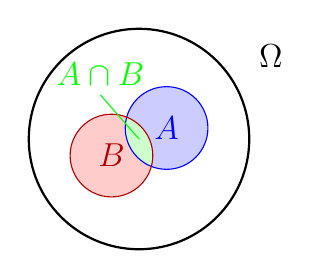
\begin{tikzpicture}[scale=0.7]
\draw[color=black,thick] (0,0) circle (2cm);
\node[color=black,right] at (2cm,1.5cm) {\large{$\Omega$}};
\fill[fill=blue!20] (0.5cm,0.2cm) circle (0.75cm);
\fill[fill=red!20] (-0.5cm,-0.3cm) circle (0.75cm);
\begin{scope}
\clip (0.5cm,0.2cm) circle (0.75cm);
\fill[fill=green!20] (-0.5cm,-0.3cm) circle (0.75cm);
\end{scope}
\draw[color=blue] (0.5cm,0.2cm) circle (0.75cm) node {\large{$A$}};
\draw[color=red!70!black] (-0.5cm,-0.3cm) circle (0.75cm) node {\large{$B$}};
\draw[color=green] (0,0)--(-0.7cm,0.8cm) node[above] {\large{$A\cap B$}};
%\fill[fill=violet!20] (2.125cm,-1.5cm) rectangle +(0.5cm,0.5cm) node[color=violet,pos=0.5,right=0.25cm] {$P$};
\end{tikzpicture}
\end{center}
\end{minipage}


\begin{minipage}{5cm}
\begin{center}
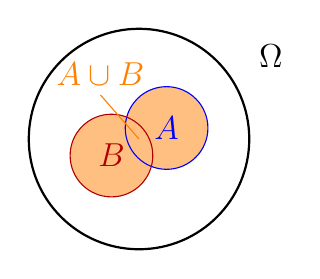
\begin{tikzpicture}[scale=0.7]
\draw[color=black,thick] (0,0) circle (2cm);
\node[color=black,right] at (2cm,1.5cm) {\large{$\Omega$}};
\fill[fill=orange!50] (0.5cm,0.2cm) circle (0.75cm);
\fill[fill=orange!50] (-0.5cm,-0.3cm) circle (0.75cm);
\begin{scope}
\clip (0.5cm,0.2cm) circle (0.75cm);
\fill[fill=orange!50] (-0.5cm,-0.3cm) circle (0.75cm);
\end{scope}
\draw[color=blue] (0.5cm,0.2cm) circle (0.75cm) node {\large{$A$}};
\draw[color=red!70!black] (-0.5cm,-0.3cm) circle (0.75cm) node {\large{$B$}};
\draw[color=orange] (0,0)--(-0.7cm,0.8cm) node[above] {\large{$A\cup B$}};
%\fill[fill=violet!20] (2.125cm,-1.5cm) rectangle +(0.5cm,0.5cm) node[color=violet,pos=0.5,right=0.25cm] {\large{$P$}};
\end{tikzpicture}
\end{center}
\end{minipage}
\begin{minipage}{9.5cm}
\textbf{Réunion d'événements} : l'événement constitué des issues appartenant à $A$ ou à $B$ est noté $A\cup B$ \\(se lit $A$ et de $B$ ou \og $A$ union $B$ \fg{} ou \og $A$ ou $B$ \fg).
\end{minipage}
\end{defi}

\begin{rem}{}{}
   Si $A\cap B=\varnothing$, on dit que les événements sont \textbf{disjoints} ou \textbf{incompatibles}.
\end{rem}

\begin{ex}{}{}
   On considère un jeu de $52$ cartes. On note $A$ l'événement \og obtenir une carte paire \fg{} et $B$ l'événement \og obtenir une carte de valeur inférieure strictement à six \fg. Calculer $A\cap B$ et $A \cup B$.
   \begin{reponse}
      \begin{itemize}
         \item[] $A\cap B=$ \og obtenir une carte paire et inférieures strictement à six \fg{} : $A \cap B=\{~2~;~4~\}$,
         \item[] $A \cup B=$ \og obtenir une carte paire ou inférieure strictement à six \fg{} : $A \cup B=\{~1~;~2~;~3~;~4~;~5~;~6~;~8~;~10~\}$.
      \end{itemize}
   \end{reponse}
\end{ex}

\section{Calcul de probabilités}
\begin{defi}{Loi de probabilités}{}
   Une \textbf{loi de probabilités} est un tableau qui associe à chaque issue $\omega\in\Omega$ un nombre $p$ entre $0$ et $1$. Ce nombre $p$ est la probabilité de l'issue $\omega$ et il indique si cette issue est souvent réalisée. La somme des probabilités vaut $1$.

   \begin{center}
   \begin{tabular}{|c||*{5}{c|}c}
         \cline{1-6}
         Issue & $\omega_1$ & $\omega_2$ & $\omega_3$ & $\omega_4$ & $\omega_5$ &\\
         \cline{1-6}
         Probabilité & $p_1$ & $p_2$ & $p_3$ & $p_4$ & $p_5$ & \qquad $p_1+p_2+\dots p_5 = 1$ \\
         \cline{1-6}
      \end{tabular}
   \end{center}
\end{defi}

\begin{defi}{Probabilité d'un événement}{}
   La \textbf{probabilité d'un événement} $A$ est un nombre entre $0$ et $1$ noté $P(A)$ qui indique si cet événement se réalise souvent lorsqu'on répète l'expérience. C'est la somme des probabilités des événements élémentaires qui le constituent.
\end{defi}

\begin{ex}{}{}
On lance un dé non pipé à six faces. La loi de probabilité associée est :
\begin{reponse}
      \begin{center}
   \begin{tabular}{|c||*{6}{c|}c}
         \cline{1-7}
         Issue & $1$ & $2$ & $3$ & $4$ & $5$ & $6$ &\\
         \cline{1-7}
         Probabilité & $1/6$ & $1/6$& $1/6$& $1/6$& $1/6$& $1/6$ & \qquad $\text{somme} = 1$ \\
         \cline{1-7}
      \end{tabular}
   \end{center}
\end{reponse}

La probabilité d'obtenir un nombre pair est égale à la probabilité d'obtenir un 2 plus la probabilité d'obtenir un 4 plus la probabilité d'obtenir un 6: $P(\{2;4;6\})=\troum{P(\{2\})+P(\{4\})+P(\{6\}) = 3/6 = 1/2}$
\end{ex}

\begin{defi}{Equiprobabilité}{}
On dit qu'il y a \textbf{équiprobabilité} lorsque tous les événements élémentaires ont la même probabilité,

% \begin{rem}{}{}
   Pour signifier qu'on est dans une situation d'équiprobabilité on a généralement dans l'énoncé une expression du type :
   \begin{itemize}
      \item  on lance un dé \textbf{non pipé};
      \item  dans une urne, il y a des boules \textbf{indiscernables} au toucher;
      \item  on rencontre au \textbf{hasard} une personne parmi \dots
   \end{itemize}
\end{defi}  
% \end{rem}

\begin{prop}{}{}
Dans une situation d'équiprobabilité, on a : $P(A) =\dfrac{\textrm{nombre d'éléments de }A}{\textrm{nombre d'éléments de }\Omega} =\dfrac{\textrm{Card}(A)}{\textrm{Card}(\Omega)}$.
\end{prop}

\begin{ex}{}{}
  On lance un dé équilibré à six faces. \\
  On considère les événements $A$ : \og obtenir un chiffre pair \fg{} et l'événement $B$ : \og obtenir un diviseur de six \fg{}.
   \begin{itemize}
      \item[] Le dé est équilibré donc on est dans une situation d'équiprobabilité,
      \item[] $A=\{~2~;~4~;~6~\}$ \quad donc, $P(A)=\dfrac{\textrm{nombre d'éléments de }A}{\textrm{nombre d'éléments de }\Omega} =\dfrac{3}{6}=\dfrac{1}{2}$
      \item[] $B=\{~1~;~2~;~3~;~6~\}$ \quad donc, $P(B)=\dfrac{\textrm{nombre d'éléments de }B}{\textrm{nombre d'éléments de }\Omega} =\dfrac{4}{6}=\dfrac{2}{3}$.
   \end{itemize}
\end{ex}

\begin{ex}{}{}

On lance une pièce de monnaie trois fois de suite, on peut schématiser cette expérience par un arbre :

\begin{center}
% Racine à Gauche, développement vers la droite
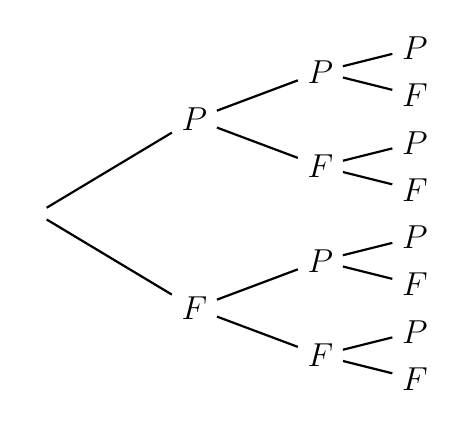
\begin{tikzpicture}[xscale=1,yscale=1,scale=0.6]
% Styles (MODIFIABLES)
\tikzstyle{fleche}=[-,>=latex,thick]
\tikzstyle{noeud}=[fill=white]
\tikzstyle{feuille}=[fill=white]
\tikzstyle{etiquette}=[midway,above]
\tikzstyle{etiquette1}=[midway,below]
% Dimensions (MODIFIABLES)
\def\DistanceInterNiveaux{2}
\def\DistanceInterFeuilles{1}
% Dimensions calculées (NON MODIFIABLES)
\def\NiveauA{(0)*\DistanceInterNiveaux}
\def\NiveauB{(1.6666666666666665)*\DistanceInterNiveaux}
\def\NiveauC{(3)*\DistanceInterNiveaux}
\def\NiveauD{(4)*\DistanceInterNiveaux}
\def\InterFeuilles{(-1)*\DistanceInterFeuilles}
% Noeuds (MODIFIABLES : Styles et Coefficients d'InterFeuilles)
\node[noeud] (R) at ({\NiveauA},{(3.5)*\InterFeuilles}) {};
\node[noeud] (Ra) at ({\NiveauB},{(1.5)*\InterFeuilles}) {\large{$P$}};
\node[noeud] (Raa) at ({\NiveauC},{(0.5)*\InterFeuilles}) {\large{$P$}};
\node[feuille] (Raaa) at ({\NiveauD},{(0)*\InterFeuilles}) {\large{$P$}};
\node[feuille] (Raab) at ({\NiveauD},{(1)*\InterFeuilles}) {\large{$F$}};
\node[noeud] (Rab) at ({\NiveauC},{(2.5)*\InterFeuilles}) {\large{$F$}};
\node[feuille] (Raba) at ({\NiveauD},{(2)*\InterFeuilles}) {\large{$P$}};
\node[feuille] (Rabb) at ({\NiveauD},{(3)*\InterFeuilles}) {\large{$F$}};
\node[noeud] (Rb) at ({\NiveauB},{(5.5)*\InterFeuilles}) {\large{$F$}};
\node[noeud] (Rba) at ({\NiveauC},{(4.5)*\InterFeuilles}) {\large{$P$}};
\node[feuille] (Rbaa) at ({\NiveauD},{(4)*\InterFeuilles}) {\large{$P$}};
\node[feuille] (Rbab) at ({\NiveauD},{(5)*\InterFeuilles}) {\large{$F$}};
\node[noeud] (Rbb) at ({\NiveauC},{(6.5)*\InterFeuilles}) {\large{$F$}};
\node[feuille] (Rbba) at ({\NiveauD},{(6)*\InterFeuilles}) {\large{$P$}};
\node[feuille] (Rbbb) at ({\NiveauD},{(7)*\InterFeuilles}) {\large{$F$}};
% Arcs (MODIFIABLES : Styles)
\draw[fleche] (R)--(Ra);
\draw[fleche] (Ra)--(Raa);
\draw[fleche] (Raa)--(Raaa);
\draw[fleche] (Raa)--(Raab);
\draw[fleche] (Ra)--(Rab);
\draw[fleche] (Rab)--(Raba);
\draw[fleche] (Rab)--(Rabb);
\draw[fleche] (R)--(Rb);
\draw[fleche] (Rb)--(Rba);
\draw[fleche] (Rba)--(Rbaa);
\draw[fleche] (Rba)--(Rbab);
\draw[fleche] (Rb)--(Rbb);
\draw[fleche] (Rbb)--(Rbba);
\draw[fleche] (Rbb)--(Rbbb);
\end{tikzpicture}

\end{center}

Chaque chemin sur cet arbre est équiprobable. On peut alors déterminer la probabilité d'obtenir 2 piles parmi 3 lancers:
\begin{reponse}
   \vspace{2cm}
\end{reponse}
\end{ex}

\begin{prop}{}{}
Soit $A$ et $B$ deux événements, on a les propriétés suivantes :

\begin{minipage}{8cm}
\begin{itemize}
\item  $P(\varnothing)=0$
\item  $P(\Omega)=1$
\end{itemize}
\end{minipage}
\begin{minipage}{9cm}
\begin{itemize}
\item  $0 \leqslant P(A) \leqslant 1$
\item  $P(\overline{A})=1-P(A)$
\item  $P(A\cup B)=P(A)+P(B)-P(A\cap B)$
\end{itemize}
\end{minipage}
\end{prop}

\begin{ex}{}{}
On considère l'ensemble $E$ des entiers de $1$ à $20$. On choisit l'un de ces nombres au hasard. \\
$A$ est l'événement : \og le nombre est multiple de $3$ \fg{} et $B$ est l'événement : \og le nombre est multiple de $2$ \fg.

\begin{align*}
   P(A) &=\troum{\dfrac{6}{20}=\dfrac{3}{10}=0,3}\\
   P(\overline{A}) &=\troum{1-P(A)=1-\dfrac{3}{10}=\dfrac{7}{10}=0,7}\\
   P(B) &=\troum{\dfrac{10}{20}=\dfrac{1}{2}=0,5}\\
   P(A \cap B)&=\troum{\dfrac{3}{20}=0,15}\\
   P(A \cup B)&=\troum{p(A)+p(B)-p(A\cap B)=\dfrac{6}{20}+\dfrac{10}{20}-\dfrac{3}{20}=\dfrac{13}{20}}
\end{align*}
\end{ex}

\newpage
\section*{Exercices}
\begin{exercices}
	\sectionexo{Loi de probabilités}
	\begin{bookexos}{43, 47, 49 p.342}\end{bookexos}
	\sectionexo{Intersection, union, complémentaire, diagramme de Venn}
	\begin{bookexos}{67, 68, 72 p.346}\end{bookexos}
   \sectionexo{Arbre de probabilités}
	\begin{bookexo}{71 p.346}\end{bookexo}
\end{exercices}
\end{document}

